\documentclass[a4paper,12pt]{article}
\usepackage{graphicx} 
\usepackage{hyperref}
\usepackage{float}
\usepackage{amsmath}
\usepackage{enumitem}
\usepackage{amsfonts}
\usepackage{booktabs}

\begin{document}

\title{Assignment 3 - Machine Learning \\
Student Placement Analysis}
\author{Mohammad Hossein Basouli}
\date{\today}
\maketitle

\section{Introduction}
In this analysis, we try to predict \textbf{student placement on a campus}, based on multiple factors; such as their \textit{Academic Data}, \textit{Demographic Information} and
\textit{Institutional Attributes}. 

\section{Data}
The dataset\cite{dataset} has been gathered by Ben Roshan D, who is doing MBA in Business Analytics at Jain University Bangalore. \\ 
It includes 215 rows and 15 features, among these 7 are categorical and 8 are numerical. 

\section{Exploratory Data Analysis}
\subsection{Data Cleaning \& Data Transformation:}
\begin{itemize}
    \item \textbf{Handling Missing Values}: Only those students that \textit{have not been place in the campus} have missing values, only in their \textit{salary} column (Figure~\ref{fig:fig_1}). 
    We will impute this by the median of this column. (Figure~\ref{fig:fig_2} shows the distribution of \textit{salary} across the two classes after the imputation.)
    \begin{figure}[H]
        \centering
        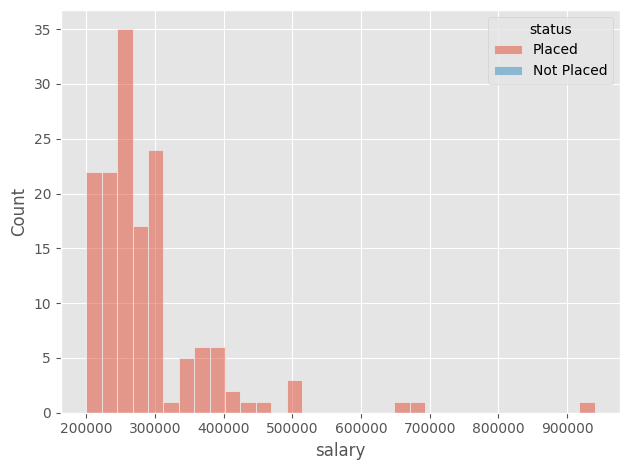
\includegraphics[width=0.7\textwidth]{./images/salary_dist_with_miss.png}
        \caption{Distribution of Salary Across The Classes Before The Imputation}
        \label{fig:fig_1}
    \end{figure}
    \begin{figure}[H]
        \centering
        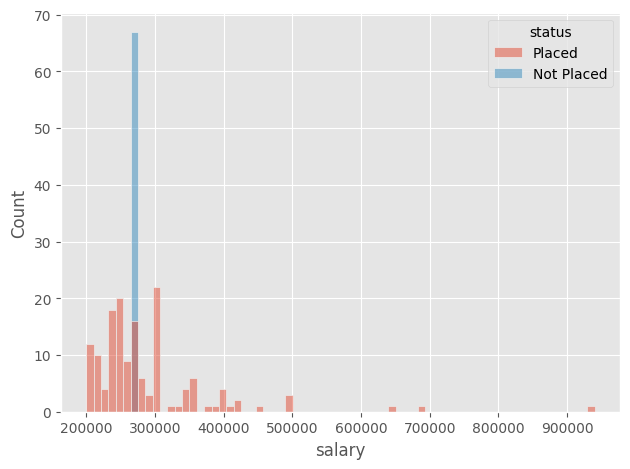
\includegraphics[width=0.7\textwidth]{./images/salary_dist_without_miss.png}
        \caption{Distribution of Salary Across The Classes After The Imputation}
        \label{fig:fig_2}
    \end{figure}
    \item \textbf{Encoding of The Categorical Features}: We will use \textbf{One-Hot Encoding} to transform our 7 categorical features into numerical.
\end{itemize}

\section{Models}

\subsection{Train \& Test Splitting:}
\%80 Train - \%20 Test 

\subsection{Threshold Tunning:}
We will use \textbf{10-Fold Stratified Cross Validation} for specifying the optimal threshold for each of our models. 

\subsection{Logistic Regression}
\subsubsection{Optimal Threshold Obtained by Cross Validation:}
Optimal threshold from CV: 0.50

\subsubsection{Model Evaluation:}

\begin{table}[H]
\centering
\caption{Logistic Regression Performance Metrics}
\begin{tabular}{lcccc}
\toprule
\textbf{Dataset} & \textbf{Accuracy} & \textbf{Precision} & \textbf{Recall} & \textbf{F1 Score} \\
\midrule
Train & 0.9012 & 0.9167 & 0.9402 & 0.9283 \\
Test  & 0.8837 & 0.9063 & 0.9355 & 0.9206 \\
\bottomrule
\end{tabular}
\end{table}

\noindent\textbf{ROC Curve}:
The \textbf{ROC Curve} for this model, evaluated on the test set, has a \textbf{Area Under The Curve} equal to 0.84, which is not that great. Also the point that the blue lines intersect
with each other, is the optimal point for \textbf{True Positive Rate} and \textbf{False Negative Rate} trade-off. \\

\noindent\textbf{Recall - Precision Curve}:
The \textbf{Recall - Precision Curve} has a \textbf{Average Precision} equal to 0.98 which is great. Also the optimal point for the trade-off of \textbf{Recall} and \textbf{Precision}
is the point where recall is around 0.82 and the curve is starting to fall. \\ 

\noindent\textbf{Confusion Matrix}:
From the \textbf{Confusion Matrix} we can see that we have misclassified 5 samples from a total of 43 samples, 2 \textbf{False Positive} and 3 \textbf{False Negatives}. \\

\begin{figure}[H]
    \centering
    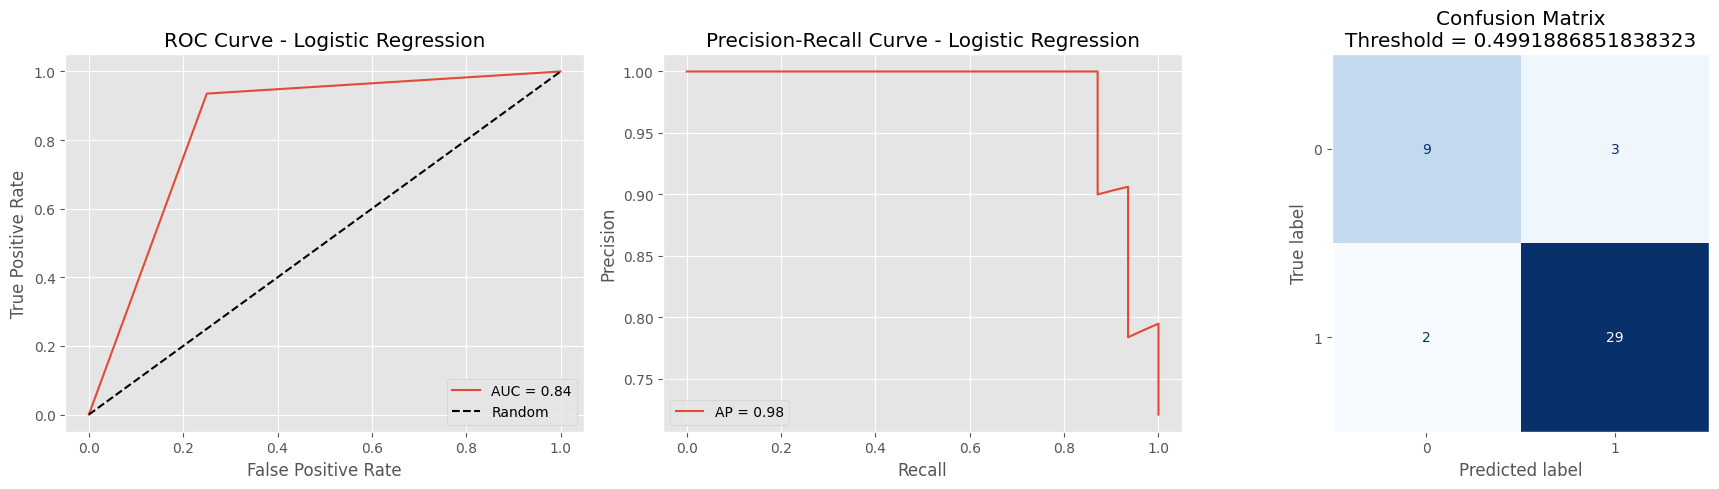
\includegraphics[width=0.7\textwidth]{./images/roc_rpc_cm_lr.png}
    \caption{ROC Curve, Recall - Precision Curve and Confusion Matrix for Logistic Regression}
    \label{fig:fig_3}
\end{figure}

\subsection{Gaussian Naive Bayes}
\subsubsection{Optimal Threshold Obtained by Cross Validation:}
Optimal threshold from CV: 1.0

\subsubsection{Model Evaluation:}

\begin{table}[H]
\centering
\caption{Gaussian Naive Bayes Performance Metrics}
\begin{tabular}{lcccc}
\toprule
\textbf{Dataset} & \textbf{Accuracy} & \textbf{Precision} & \textbf{Recall} & \textbf{F1 Score} \\
\midrule
Train & 0.9651 & 1.0000 & 0.9487 & 0.9737 \\
Test  & 1.0000 & 1.0000 & 1.0000 & 1.0000 \\
\bottomrule
\end{tabular}
\end{table}

\noindent\textbf{ROC Curve}:
The two lines intersect at a right angle, which is the optimal point for the trade-off of \textbf{True Positive Rate} and \textbf{False Negative Rate}. The \textbf{Area Under The Curve} is 1.0, which is the best that we can hope for. This indicates that the model is perfectly capable of distinguishing between the two classes. \\

\noindent\textbf{Recall - Precision Curve}:
The \textbf{Recall - Precision Curve} also shows a perfect \textbf{Average Precision} of 1.0. The curve stays at maximum precision for all recall levels until the very end, suggesting excellent performance in class separation. \\

\noindent\textbf{Confusion Matrix}:
From the \textbf{Confusion Matrix}, we observe that all 43 samples were classified correctly. There are \textbf{0 False Positives} and \textbf{0 False Negatives}, indicating perfect performance on the test set. \\

\begin{figure}[H]
    \centering
    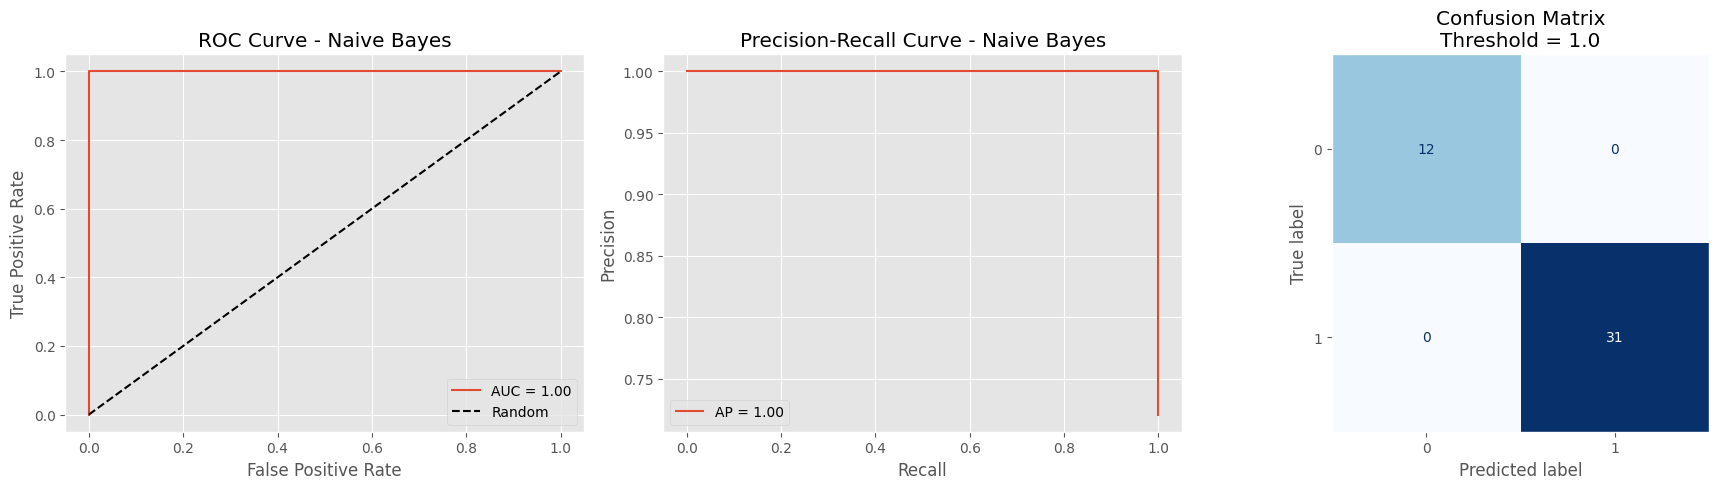
\includegraphics[width=0.7\textwidth]{./images/roc_rpc_cm_nb.png}
    \caption{ROC Curve, Recall - Precision Curve and Confusion Matrix for Gaussian Naive Bayes}
    \label{fig:fig_4}
\end{figure}


\subsection{Linear Discriminant Analysis}
\subsubsection{Optimal Threshold Obtained by Cross Validation:}
Optimal threshold from CV: 0.638

\subsubsection{Model Evaluation:}

\begin{table}[H]
\centering
\caption{Linear Discriminant Analysis Performance Metrics}
\begin{tabular}{lcccc}
\toprule
\textbf{Dataset} & \textbf{Accuracy} & \textbf{Precision} & \textbf{Recall} & \textbf{F1 Score} \\
\midrule
Train & 0.9012 & 0.9310 & 0.9231 & 0.9270 \\
Test  & 0.8605 & 0.9032 & 0.9032 & 0.9032 \\
\bottomrule
\end{tabular}
\end{table}

\noindent\textbf{ROC Curve}:
The \textbf{ROC Curve} shows an \textbf{Area Under The Curve} of 0.83, which is slightly less than ideal but still fairly strong. The curve indicates a good separation between the classes, although not as pronounced as in Naive Bayes. \\ 

\noindent\textbf{Recall - Precision Curve}:
The \textbf{Recall - Precision Curve} has a high \textbf{Average Precision} of 0.98, suggesting the model performs well in terms of maintaining high precision even as recall increases. The curve begins to slightly fall around a recall of 0.82, which marks a reasonable trade-off point. \\

\noindent\textbf{Confusion Matrix}:
The \textbf{Confusion Matrix} reveals that 6 out of 43 samples were misclassified: 3 \textbf{False Positives} and 3 \textbf{False Negatives}. While the model performs well overall, there is a small number of errors that might be worth addressing depending on the application. \\ 

\begin{figure}[H]
    \centering
    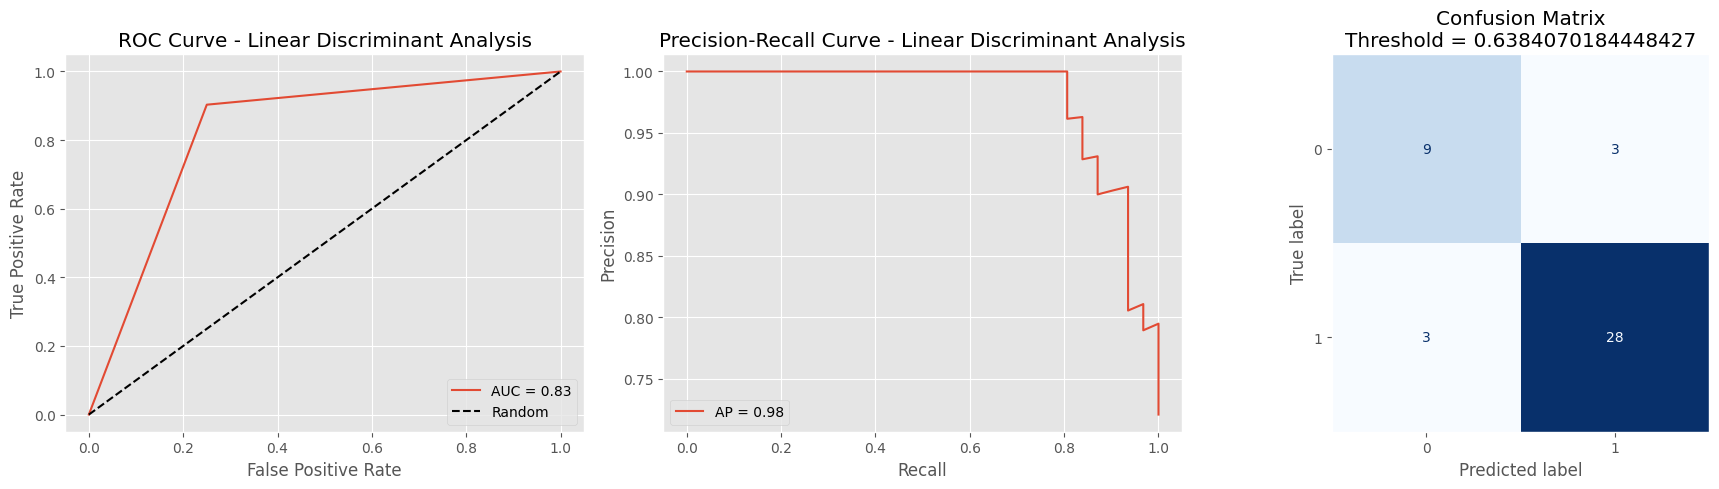
\includegraphics[width=0.7\textwidth]{./images/roc_rpc_cm_lda.png}
    \caption{ROC Curve, Recall - Precision Curve and Confusion Matrix for Linear Discriminant Analysis}
    \label{fig:fig_5}
\end{figure}


\subsection{Best Model:}
\textbf{Gaussian Naive Bayes} performs better in all aspects. 


\begin{thebibliography}{9}

\bibitem{dataset}
Campus Recruitment, \textit{Academic and Employability Factors influencing placement}, \\
Available at: \url{https://www.kaggle.com/datasets/benroshan/factors-affecting-campus-placement/data}, 2020.

\end{thebibliography}

\end{document}